\documentclass[10pt,letterpaper]{article}
\usepackage[top=0.85in,left=2.75in,footskip=0.75in,marginparwidth=2in]{geometry}

% use Unicode characters - try changing the option if you run into troubles with special characters (e.g. umlauts)
\usepackage[utf8]{inputenc}
\usepackage{threeparttable}

% clean citations
\usepackage{cite}

% hyperref makes references clicky. use \url{www.example.com} or \href{www.example.com}{description} to add a clicky url
\usepackage{nameref,hyperref}

% line numbers
\usepackage[right]{lineno}

% improves typesetting in LaTeX
\usepackage{microtype}
\DisableLigatures[f]{encoding = *, family = * }

% text layout - change as needed
\raggedright
\setlength{\parindent}{0.5cm}
\textwidth 5.25in 
\textheight 8.75in

% Remove % for double line spacing
%\usepackage{setspace} 
%\doublespacing

% use adjustwidth environment to exceed text width (see examples in text)
\usepackage{changepage}

% adjust caption style
\usepackage[aboveskip=1pt,labelfont=bf,labelsep=period,singlelinecheck=off]{caption}

% remove brackets from references
\makeatletter
\renewcommand{\@biblabel}[1]{\quad#1.}
\makeatother

% headrule, footrule and page numbers
\usepackage{lastpage,fancyhdr,graphicx}
\usepackage{epstopdf}
\pagestyle{myheadings}
\pagestyle{fancy}
\fancyhf{}
\rfoot{\thepage/\pageref{LastPage}}
\renewcommand{\footrule}{\hrule height 2pt \vspace{2mm}}
\fancyheadoffset[L]{2.25in}
\fancyfootoffset[L]{2.25in}

% use \textcolor{color}{text} for colored text (e.g. highlight to-do areas)
\usepackage{color}

% define custom colors (this one is for figure captions)
\definecolor{Gray}{gray}{.25}

% this is required to include graphics
\usepackage{graphicx}

% use if you want to put caption to the side of the figure - see example in text
\usepackage{sidecap}

% use for have text wrap around figures
\usepackage{wrapfig}
\usepackage[pscoord]{eso-pic}
\usepackage[fulladjust]{marginnote}
\reversemarginpar

\begin{document}
\vspace*{0.35in}

% title goes here:
\begin{flushleft}
{\Large
\textbf\newline{Supplemental Material: Evaluating trait-based sets for taxonomic enrichment analysis applied to human microbiome data sets}
}
\newline
% authors go here:
\\
Quang P. Nguyen\textsuperscript{1,2,*},
Anne G. Hoen\textsuperscript{1,2,+.*},
H. Robert Frost\textsuperscript{2,+,*}
\\
\bigskip
\bf{1} Department of Epidemiology, Geisel School of Medicine at Dartmouth College
\\
\bf{2} Department of Biomedical Data Science, Geisel School of Medicine at Dartmouth College
\\
\bigskip
+ These authors jointly supervised this research \\

* Co-corresponding authors: quangpmnguyen@gmail.com, hildreth.r.frost@dartmouth.edu, anne.g.hoen@dartmouth.edu

\end{flushleft}



\begin{figure}[!h]
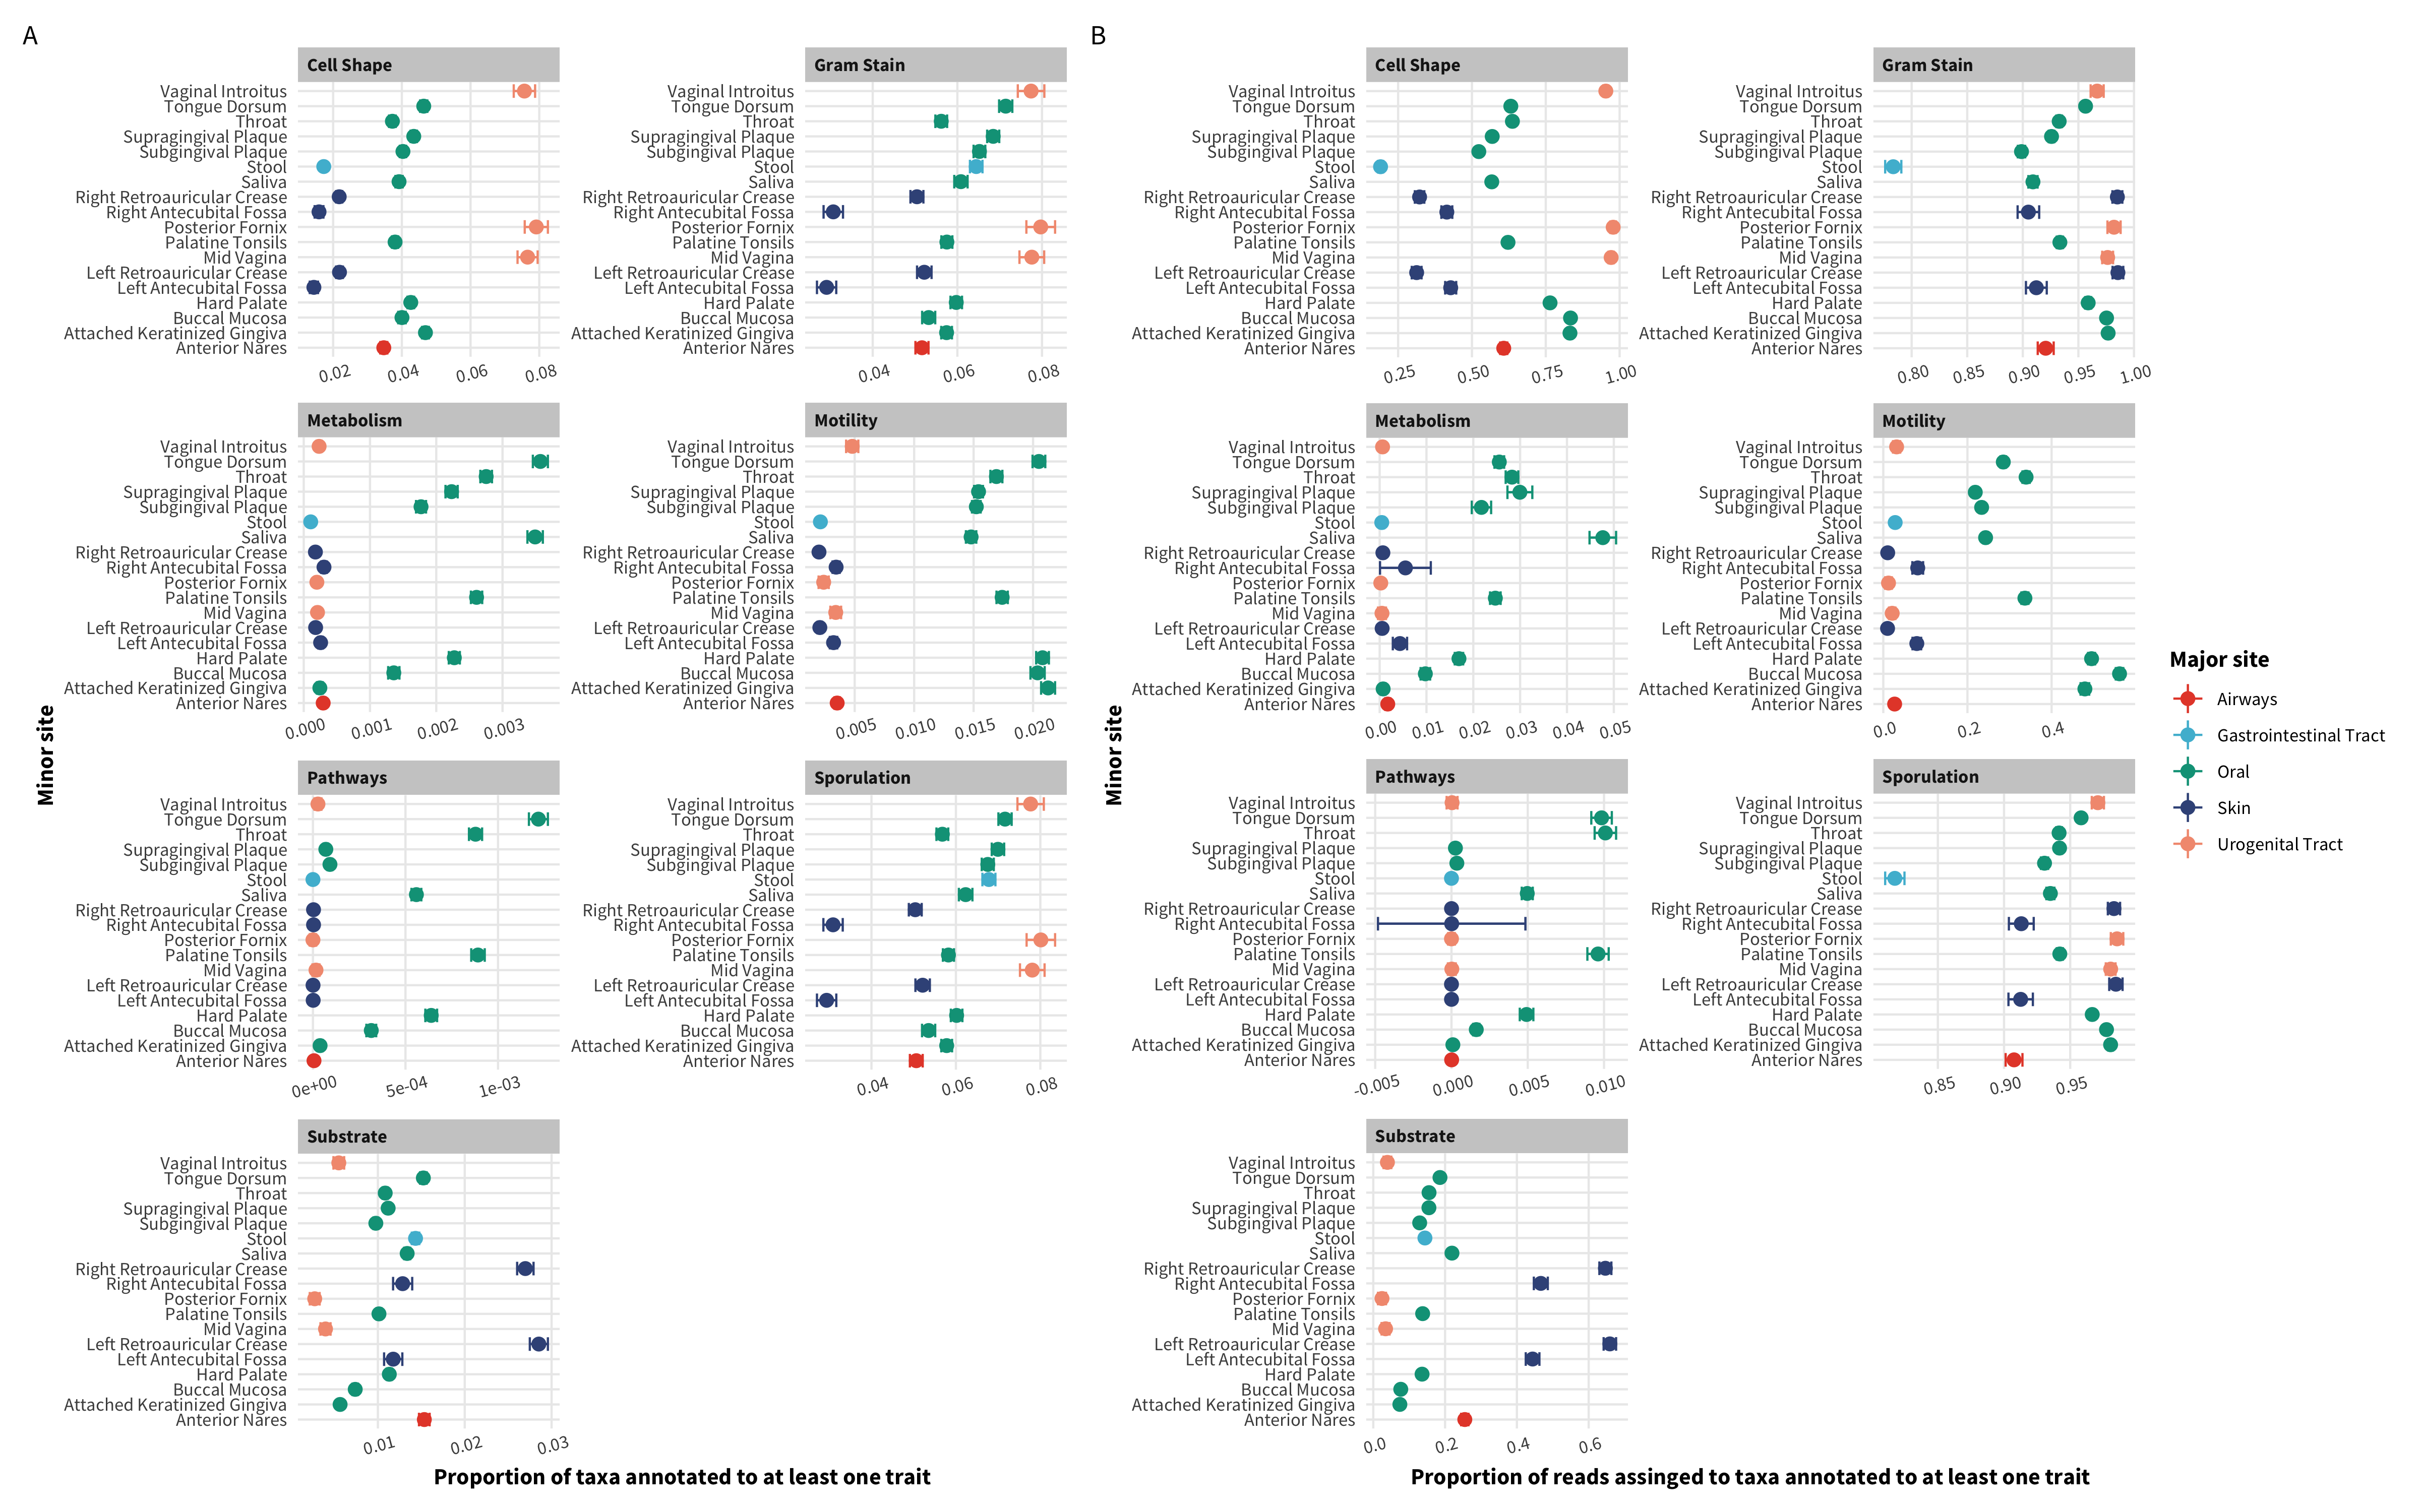
\includegraphics[width=0.99\linewidth]{figures/coverage_16s.png}
\caption{Trait coverage statistics for samples profiled with 16S rRNA gene metabarcoding. Panel \textbf{(A)} illustrates the proportion of present taxa per sample annotated to at least one trait. Panel \textbf{(B)} illustrates the proportion of reads assigned to taxa annotated to at least one trait which accounts for taxa relative abundances. Each plot facet represents different trait categories that were evaluated. Error bar represents the standard error of the evaluation statistic of interest across the the total number of samples evaluated per body site.}
\label{fig:s1}
\end{figure}


\begin{figure}[!h]
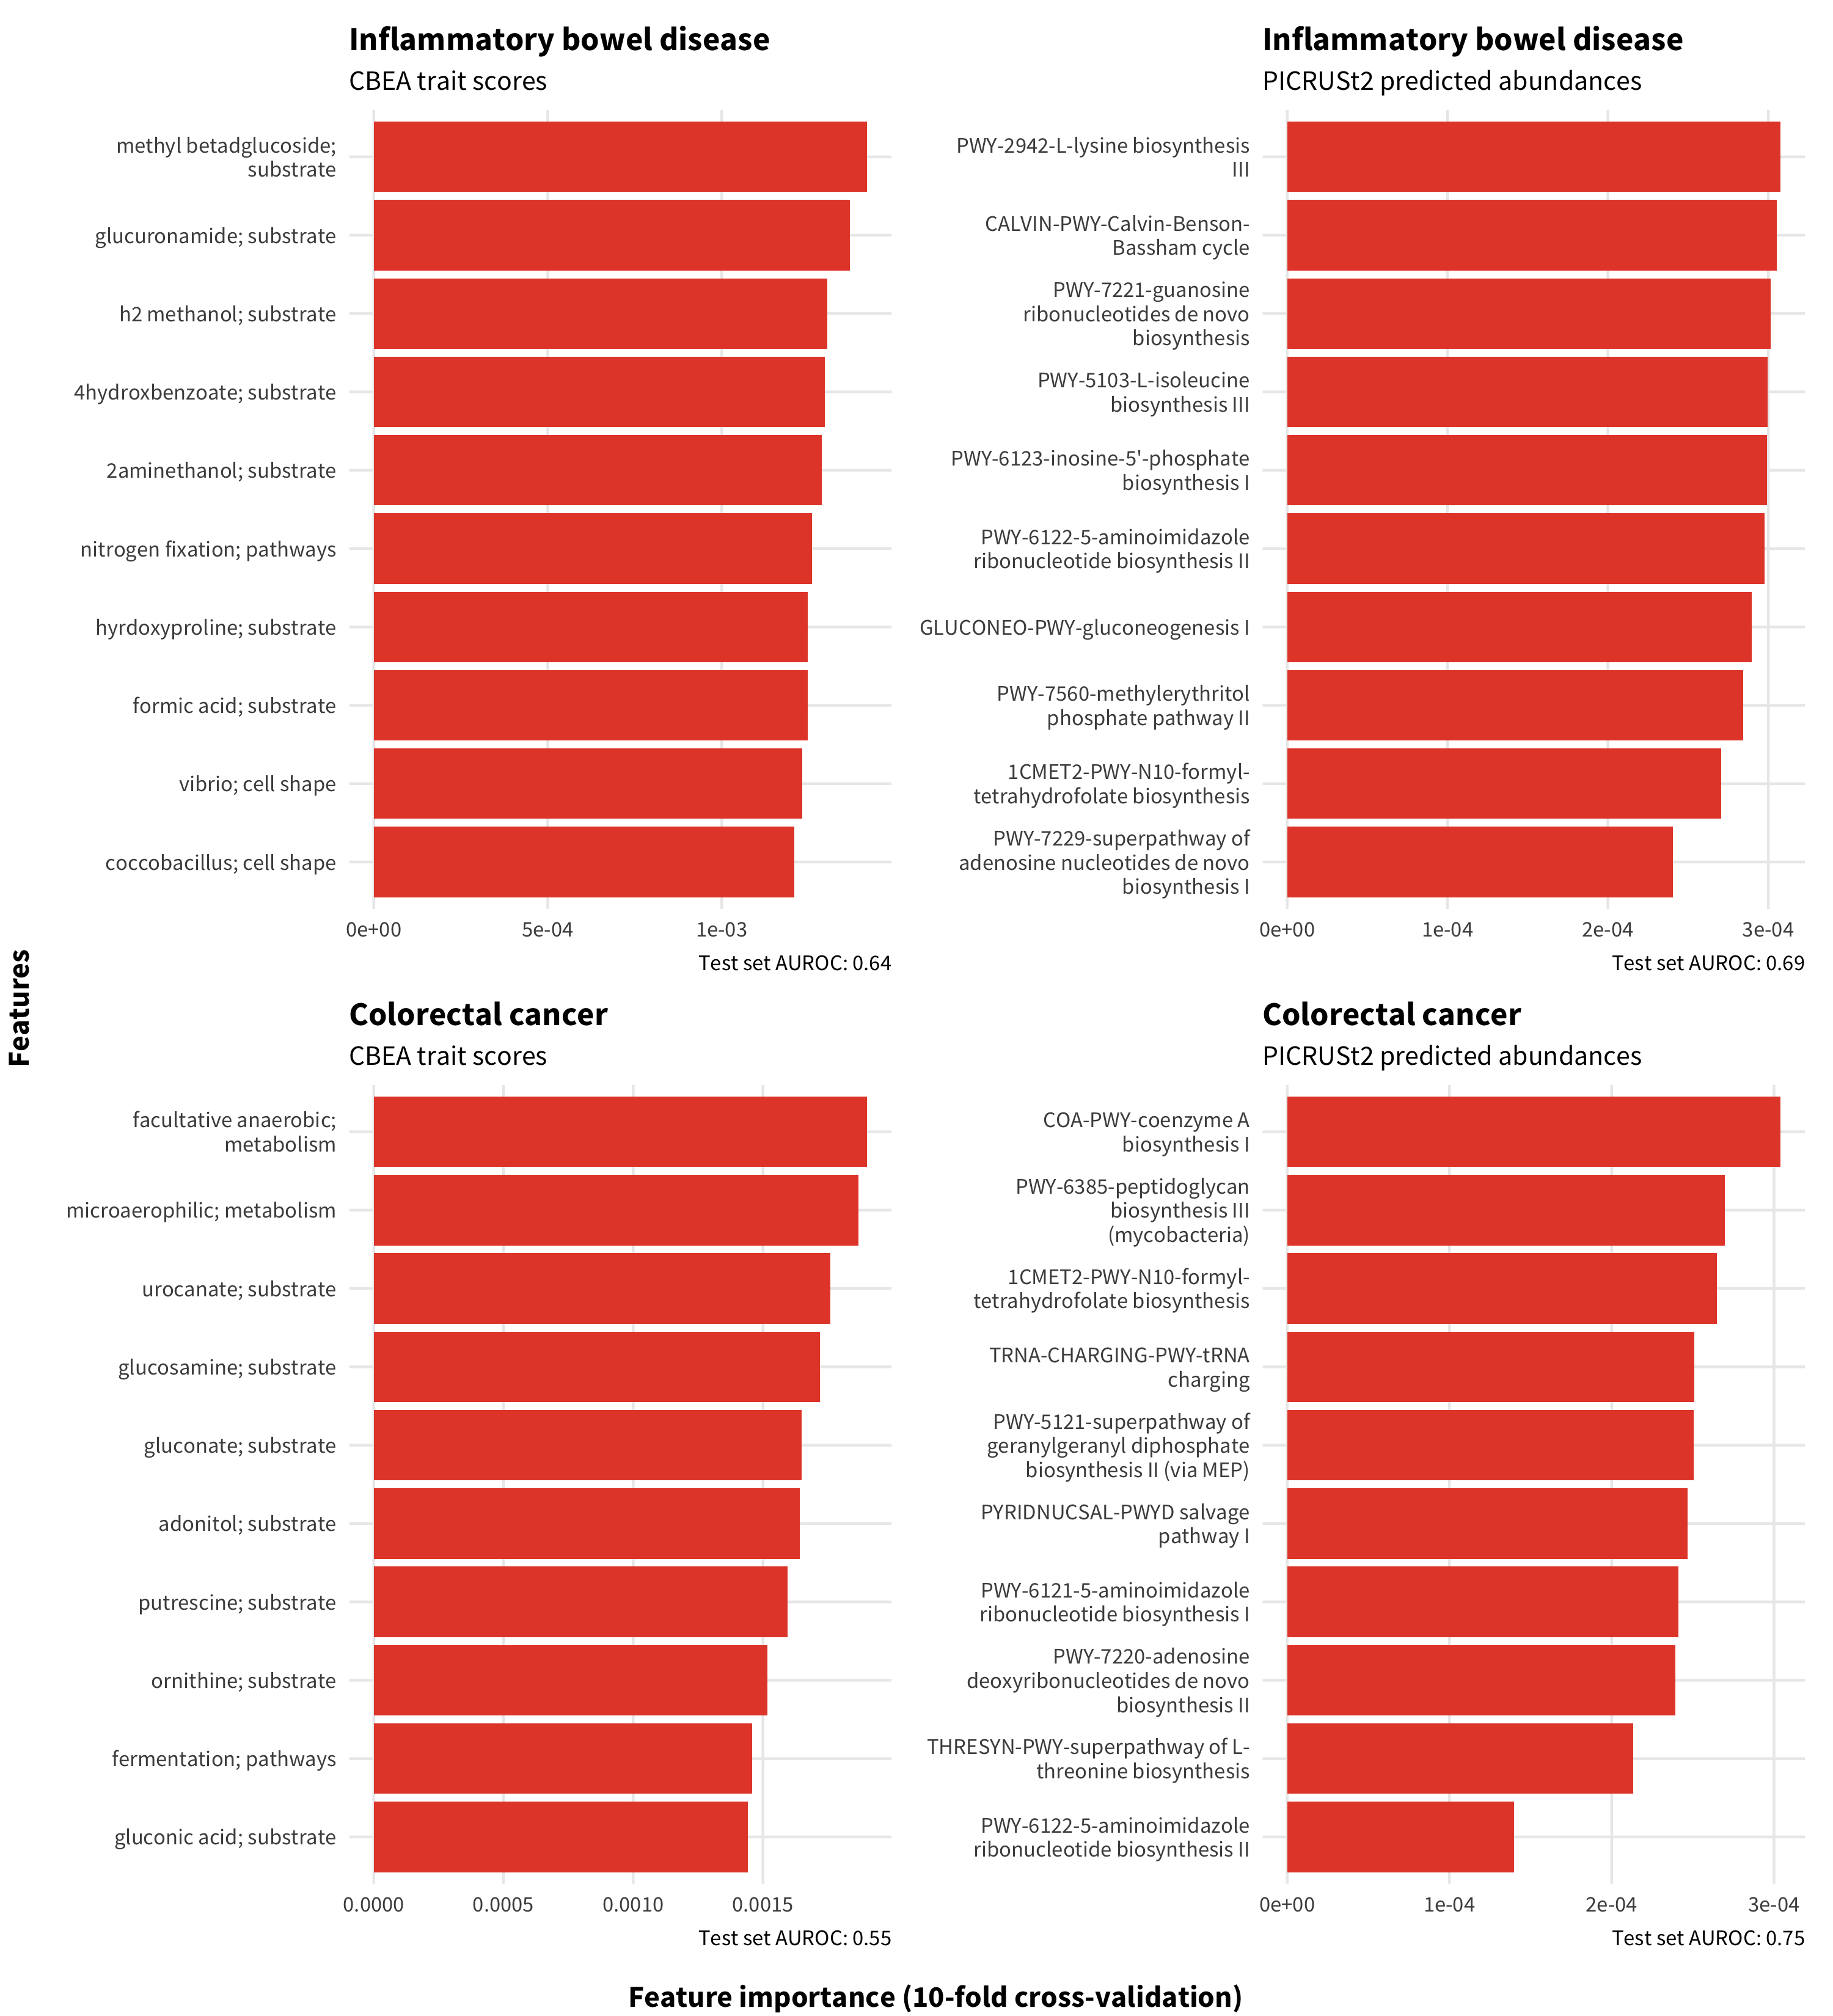
\includegraphics[width=0.99\linewidth]{figures/feat_importance_16s.png}
\caption{Top 10 important features based on random forest model fitted on different inputs from data sets profiled with 16S rRNA gene sequencing.  Features were selected from mean decrease in Gini impurity averaged across 500 decision trees and 10-fold cross-validation (nested with the training set) as implemented in \texttt{scikit-learn}. AUROC scored on a held-out test set is also presented for each input type and disease condition.}
\label{fig:s2}
\end{figure}


\end{document}

\section*{Appendix}
\paragraph*{S1 Fig.}
\label{S1_Fig}
{\bf Trait coverage statistics for samples profiled with 16S rRNA gene metabarcoding.} Panel \textbf{(A)} illustrates the proportion of present taxa per sample annotated to at least one trait. Panel \textbf{(B)} illustrates the proportion of reads assigned to taxa annotated to at least one trait which accounts for taxa relative abundances. Each plot facet represents different trait categories that were evaluated. Error bar represents the standard error of the evaluation statistic of interest across the the total number of samples evaluated per body site.

\paragraph*{S2 Fig.}
\label{S2_Fig}
{\bf Top 10 important features based on random forest model fitted different inputs from data sets profiled with 16S rRNA gene sequencing}. Features were selected from mean decrease in Gini impurity averaged across 500 decision trees and 10-fold cross-validation (nested with the training set) as implemented in \texttt{scikit-learn}. AUROC scored on a held-out test set is also presented for each input type and disease condition.


\section*{Additional Files}
  \subsection*{Fig S1 --- \textbf{Trait coverage statistics for samples profiled with 16S rRNA gene metabarcoding}. Panel \textbf{(A)} illustrates the proportion of present taxa per sample annotated to at least one trait. Panel \textbf{(B)} illustrates the proportion of reads assigned to taxa annotated to at least one trait which accounts for taxa relative abundances. Each plot facet represents different trait categories that were evaluated. Error bar represents the standard error of the evaluation statistic of interest across the the total number of samples evaluated per body site.}
  \subsection*{Fig S2 --- \textbf{Top 10 important features based on random forest model fitted on different inputs from data sets profiled with 16S rRNA gene sequencing}.  Features were selected from mean decrease in Gini impurity averaged across 500 decision trees and 10-fold cross-validation (nested with the training set) as implemented in \texttt{scikit-learn}. AUROC scored on a held-out test set is also presented for each input type and disease condition.}